\documentclass[border=10pt]{standalone}
% \documentclass{article}
\usepackage{tikz}
\usetikzlibrary{arrows,decorations.pathmorphing,backgrounds,positioning,fit,petri,patterns}
\tikzstyle{particle} = [thick, fill=black!10]

\usepackage[T1]{fontenc}
\usepackage{dsfont}
\usepackage[utopia, greeklowercase=upright]{mathdesign}
\usepackage{amsmath}

\begin{document}

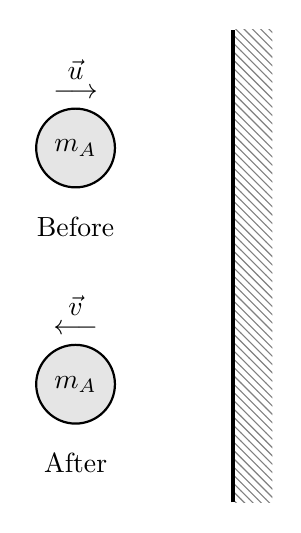
\begin{tikzpicture}

\fill[pattern=north west lines, pattern color=black!50, draw=none] (2,-3) rectangle (2.5,3);
\draw[ultra thick] (2,-3) -- (2,3);

\draw[particle] (0,1.5) circle (0.5) node {$m_{A}$}
	+ (0,0.5) node[above] {$\longrightarrow$}
	+ (0,1) node {$\vec{u}$}
	+ (0,-1) node[align=center] {Before}	
;

\draw[particle] (0,-1.5) circle (0.5) node {$m_{A}$}
	+ (0,0.5) node[above] {$\longleftarrow$}
	+ (0,1) node {$\vec{v}$}
	+ (0,-1) node[align=center] {After}	
;

\end{tikzpicture}

\end{document}